In the basic theory of quantum error correction, quantum states are encoded into
several highly entangled physical qubits. By performing the appropriate parity
checks, it is possible to probe the state of the physical qubits without
changing the state of the encoded qubit (also called the \textit{logical
  qubit}), in order to detect errors on individual physical qubits. These parity
checks are the \textit{stabilizers} of the error correction code; when all
stabilizer measurements return an eigenvalue of $+1$, it signals that no error
has occurred \cite{nielsen_chuang_2010}. Effective encoding protocols are
constructed such that that each error process gives rise to a unique syndrome,
which is just the list of stabilizer measurement outcomes, which provides the
information needed to correct the error \cite{fowler12_surfac_codes}.

%move to FT section?
In any real implementation of physical qubits, there are several sources of
error. State preparation and measurement may not be carried out perfectly.
Coherent errors also occur through the imperfect application of quantum gates in
circuits \cite{Devitt_2013}. Error models and error correction schemes are all
predicated on the assumption that low-weight errors (affecting only a few
qubits) are more likely than high weight errors. In other words, error
probabilities must be small \cite{terhal15}. In principle though, all these
(unlikely) sources of error can be corrected for using a variety of encoding and
detection schemes.

The error detection scheme implemented by the surface code, shown in Fig.
\ref{fig:surface_code}, is capable of precisely identifying errors in large
arrays of qubits. The $X$- and $Z$-stabilizer ancillas conduct parity
measurements between the data qubits to which they are connected through a
sequence of controlled-not (CNOT) operations. Should an error occur on a given
data qubit, depending on the error type ($X$, $Y$, or $Z$) either the $X$ or $Z$
(or both) type stabilizers will fire (return an outcome of $-1$ in their
measurement), which heralds the error and allows for its appropriate correction.
Corrections often take place at the software level, since applications of gates
in the hardware are susceptible to noise. It is often easier (and less
error-prone) to propagate the error through the circuit and correct the outcome
of a measurement than it is to physically correct the error in the hardware.

\subsection{Fault tolerance}
As mentioned in the previous section, errors can occur at every point in the
execution of an algorithm. State preparation, measurement, and gate operations
are examples of operations that are affected by these errors. Furthermore, the
errors occurring at any of these steps may propagate through the different
operations to the rest of the components of the system. This could lead to
cascading errors throughout the entire process, destroying all reliability in
the computation through loss of coherence. If a quantum computer is ever to be
realized, errors must be carefully contained.

It is in this context of error propagation that the concept of
\textit{fault-tolerant} quantum computing arises. A certain operation is said to
be fault-tolerant if a single error occurring at any step between two QEC cycles
causes at most one error at each of the logical blocks involved in the operation
\cite{Devitt_2013}. An example of fault-tolerant operation is shown in Fig.
\ref{fig:fault_tol} (b) where a bit-flip error in the top logical block
propagates only once to the bottom logical block (in contrast to (a) where it
propagates multiply). It is noteworthy that the constraint of only one
error propagating to different logical blocks can be relaxed when increasing the
code distance \cite{Devitt_2013}. In fact, for codes of distance $d$, it suffices
to require $d-2$ errors at each logical block.

\begin{figure}[htbp]
  \centering
  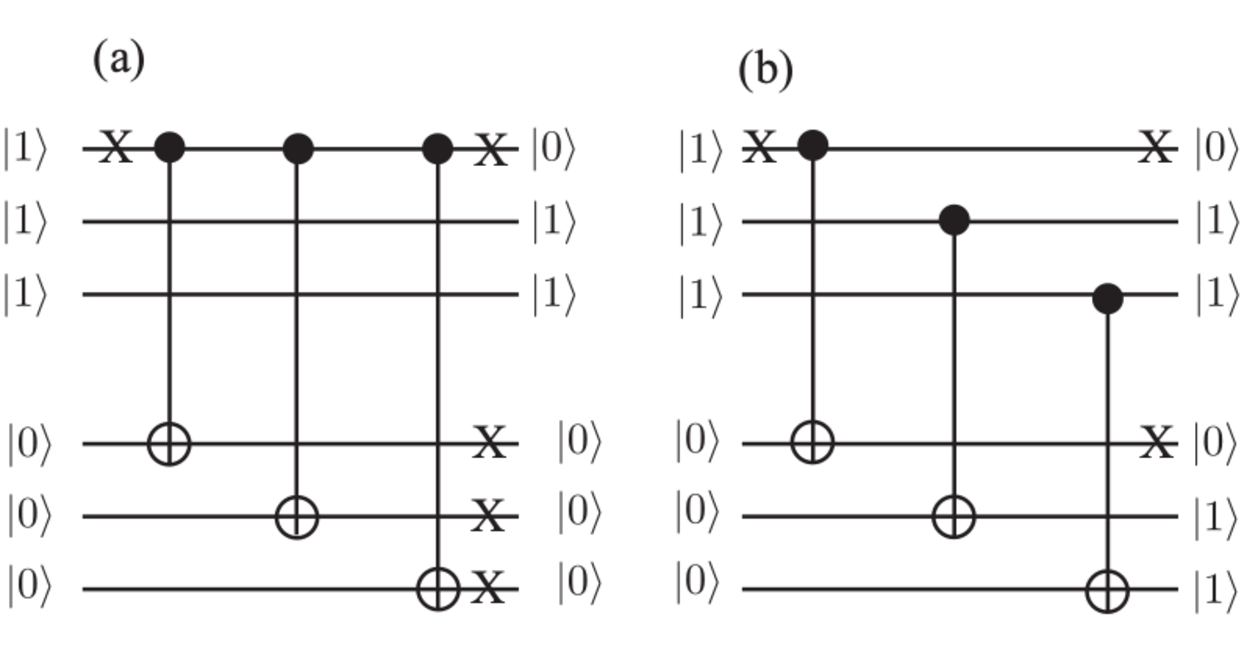
\includegraphics[width=0.5\textwidth]{images/fault_tolerance.pdf}
  \caption{Exmple of an operation that is not fault-tolerant (a) and one that is
    fault-tolerant (b). In these examples a bit-flip error in the top logical
    block propagates through the CNOT gates to the bottom logical block.}
  \label{fig:fault_tol}
\end{figure}

\subsection{Decoding Algorithms}
Once the error syndrome is known, it is necessary to perform a decoding process
to obtain the best guess for what error occurred. Optimally decoding such
syndromes is an NP-complete problem, and therefore no efficient (polynomial
time) algorithm yet exists \cite{Berlekamp}. However, the main challenge still
consists in obtaining a fast yet precise algorithm, which is preferably scalable
with the number of data qubits. As mentioned, book-keeping errors at the
software level allows for corrections to be applied at the end of the
computation process by adapting the measurement output of the data qubits.

We would like to mention two different approaches. The \textit{maximum
  likelihood method} \cite{Varsamopoulos_2020} finds and applies the most
probable correction consistent with a given error model. It features high
accuracy but low efficiency. Another popular approach uses the \textit{minimum
  weight perfect matching} \cite{fowler2013minimum} algorithm. In this case,
error syndromes are represented as a weighted graph. Afterwards, the vertices of
this graph are paired minimizing their total weight. This pairing establishes
the operation necessary to correct the error. The minimum weight perfect
matching protocol greatly increases decoding speed at a modest cost for the
accuracy.

\subsection{Error threshold}
One great strength of the surface code is its ability to diagnose multiple
errors simultaneously. Should two adjacent $X$-checks fire at one end of the
surface, while two $Z$-checks fire at the other end, we can conclude that a
phase-flip error occurred on the data qubit between the two $X$-checks, while a
bit-flip error occurred between the $Z$-checks. One must be careful, however,
because decoding the error syndrome for any code is a problem without a unique
solution \cite{terhal15}. Taking the top-left data qubit in Fig.
\ref{fig:surface_code} as an example, one can confirm that a bit-flip error on
that qubit would give rise to the exact same syndrome as a series of bit-flip
errors on the rest of the top row of data qubits. For systems with small error
probabilities, the single bit-flip error is of course much more likely than the
long series of errors required to produce the same syndrome, but as the error
rate grows, such mistakes in identifying the cause of a syndrome become more
commonplace.

When a syndrome is misinterpreted, the code implements the \textit{wrong
  correction}, and this can lead to a logical level operation being applied to
the logical qubit. The rate at which this occurs, called the \textit{logical
  error rate}, as a function of the physical error rate of the code is of great
interest in characterizing the effectiveness of an error correction protocol.

Indeed, we want the logical error rate to decrease as a function of increasing
code distance, either by means of concatenation or, in the case of surface
codes, by increasing the dimensions of surface. However, a high error rate would
prevent this from happening. In the case of surfaces codes, a simple empirical
equation that encapsulates the main properties of the logical error rate
obtained in simulations is \cite{fowler12_surfac_codes}
\begin{equation}
  \label{eq:1}
  P_L = c\left(\frac{p}{p_{th}}\right)^{\frac{ d+1 }{2}},
\end{equation}
where $d$ is the distance of the QEC protocol employed, $c$ is a constant that
depends on the exact characteristics of the error model, $p$ is the physical
error rate under sensible assumptions and $p_{th}$ is the error rate threshold.
This equation clearly shows that the process of encoding is beneficial (leads to
a lower logical error rate) only if the physical qubit error rate is below the
critical threshold value of $p_{th}$. Even though these threshold error rates
vary depending on the employed error model, the current consensus puts the
threshold at around $1\%$ \cite{terhal15} \cite{Versluis_2017}. However,
achieving a physical system that accomplishes such a low error rate
experimentally remains an outstanding challenge.

%%% Local Variables:
%%% mode: latex
%%% TeX-master: "QEC_paper"
%%% End: